%%
%%  Annexes
%%
%%  Note: Ne pas modifier la ligne ci-dessous. / Do not modify the following line.
\ifthenelse{\equal{\Langue}{english}}{
	\addcontentsline{toc}{compteur}{APPENDICES}
}{
	\addcontentsline{toc}{compteur}{ANNEXES}
}



\Annexe{ARTICLE}

On inclut à la page suivante l'article \href{https://dl.acm.org/doi/10.1145/3391274.3393637}{\textit{What is the Schema of your Knowledge Graph: Leveraging Knowledge Graph Embeddings and Clustering for Expressive Taxonomy Learning}}, co-écrit avec Amal Zouaq et présenté à la conférence SBD 2020. Son contenu correspond aux chapitres \ref{chap:kge} et \ref{chap:texp} du présent mémoire.
% \textit{International Workshop  on Semantic Big Data} 2020

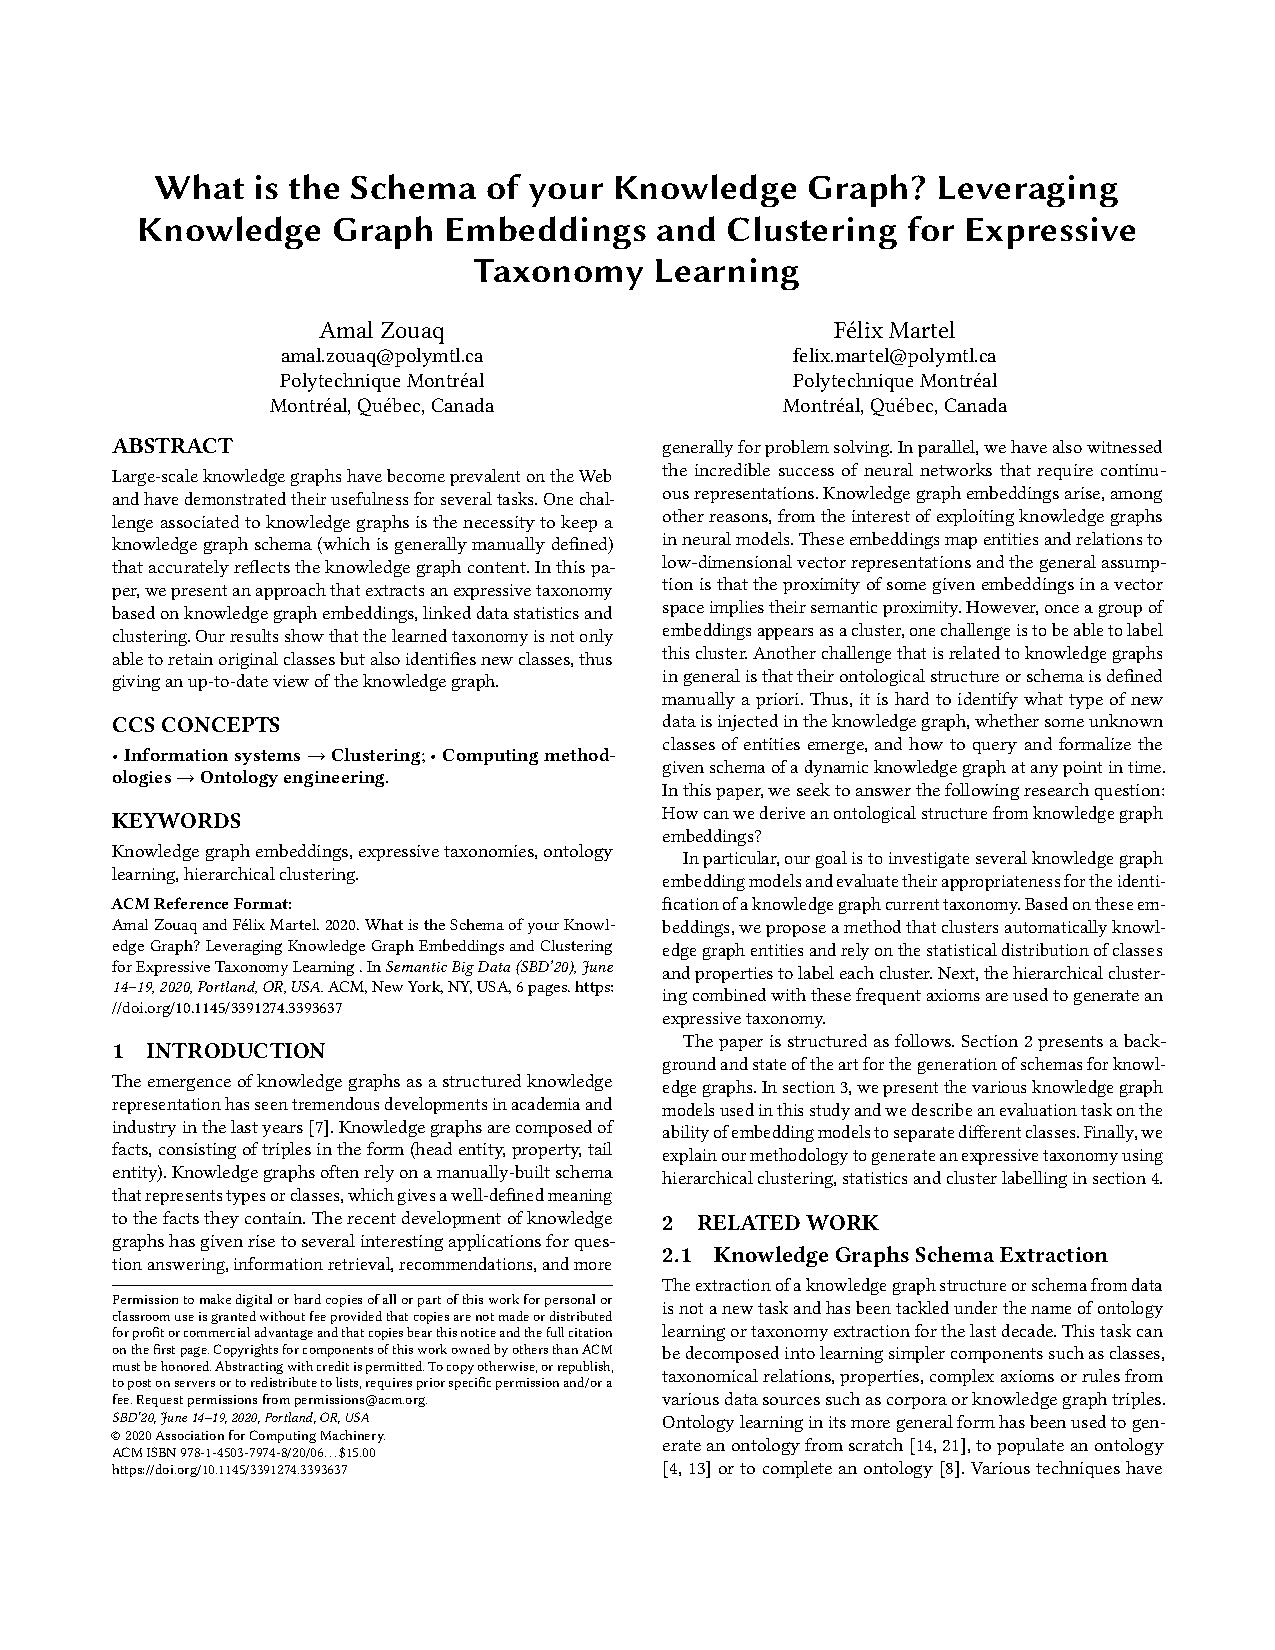
\includepdf[pages=-]{sigmod-article.pdf}


\Annexe{RÉSULTATS COMPLETS POUR L'EXTRACTION DE TAXONOMIE}
\label{ann:results}
Le tableau \ref{tab:te-full-results} présente les résultats complets de l'extraction de taxonomie, et inclut notamment les modèles, les métriques et les critères de liaison qui ont été omis à la section \ref{subsec:te-results}. Dans ce tableau, «cos», «euc», «l1» désignent respectivement les distances cosinus, euclidienne et $L_1$, tandis que «max», «min», «moy» et «ward» désignent le saut maximum, le saut minimum, le saut moyen et le critère de Ward.
%\begin{table}[htbp]
%\centering
%\caption{Caption}
%\label{tab:my_label}
\begin{longtable}{|llll|ccc|ccc|}
    \caption{Résultats complets pour l'extraction de taxonomie présentée à la section \ref{subsec:te-results}.}
    \label{tab:te-full-results}
    \hline 
	&		&		&		&	\multicolumn{3}{c|}{Directe} & \multicolumn{3}{c|}{Transitive}   \\
Plongements	&	Méthode	&	Métrique	&	Liaison	&	$p$	&	$r$	&	$F_1$	&	$p$	&	$r$	&	$F_1$	\\
\hline \endhead
\hline \endfoot
ComplEx	&	MLI	&	cos	&	max	&	0.47	&	0.38	&	0.42	&	0.77	&	0.5	&	0.61 \\ 
ComplEx	&	MLI	&	euc	&	max	&	0.4	&	0.36	&	0.38	&	0.73	&	0.53	&	0.62 \\ 
ComplEx	&	MLI	&	l1	&	max	&	0.38	&	0.33	&	0.35	&	0.68	&	0.57	&	0.62 \\ 
DistMult	&	MLI	&	cos	&	max	&	0.49	&	0.41	&	0.44	&	0.65	&	0.53	&	0.59 \\ 
DistMult	&	MLI	&	euc	&	max	&	0.29	&	0.23	&	0.26	&	0.52	&	0.42	&	0.46 \\ 
DistMult	&	MLI	&	l1	&	max	&	0.26	&	0.19	&	0.22	&	0.49	&	0.36	&	0.42 \\ 
RDF2Vec	&	MLI	&	cos	&	max	&	0.3	&	0.23	&	0.26	&	0.58	&	0.35	&	0.44 \\ 
RDF2Vec	&	MLI	&	euc	&	max	&	0.5	&	0.3	&	0.37	&	0.79	&	0.35	&	0.49 \\ 
RDF2Vec	&	MLI	&	l1	&	max	&	0.29	&	0.31	&	0.3	&	0.48	&	0.54	&	0.51 \\ 
TransD	&	MLI	&	cos	&	max	&	0.05	&	0.05	&	0.05	&	0.19	&	0.21	&	0.2 \\ 
TransD	&	MLI	&	euc	&	max	&	0	&	0	&	0	&	0.11	&	0.22	&	0.15 \\ 
TransD	&	MLI	&	l1	&	max	&	0.06	&	0.06	&	0.06	&	0.18	&	0.3	&	0.23 \\ 
TransE	&	MLI	&	cos	&	max	&	0.76	&	0.64	&	0.69	&	0.92	&	0.64	&	0.75 \\ 
TransE	&	MLI	&	euc	&	max	&	0.55	&	0.48	&	0.52	&	0.86	&	0.53	&	0.66 \\ 
TransE	&	MLI	&	l1	&	max	&	0.72	&	0.64	&	0.68	&	0.94	&	0.58	&	0.72 \\ 
ComplEx	&	MLM	&	cos	&	max	&	0.51	&	0.39	&	0.44	&	0.86	&	0.57	&	0.69 \\ 
ComplEx	&	MLM	&	euc	&	max	&	0.42	&	0.34	&	0.38	&	0.81	&	0.57	&	0.67 \\ 
ComplEx	&	MLM	&	l1	&	max	&	0.42	&	0.31	&	0.36	&	0.84	&	0.55	&	0.67 \\ 
DistMult	&	MLM	&	cos	&	max	&	0.46	&	0.39	&	0.42	&	0.9	&	0.61	&	0.73 \\ 
DistMult	&	MLM	&	euc	&	max	&	0.45	&	0.36	&	0.4	&	0.84	&	0.55	&	0.67 \\ 
DistMult	&	MLM	&	l1	&	max	&	0.33	&	0.17	&	0.23	&	0.7	&	0.31	&	0.43 \\ 
RDF2Vec	&	MLM	&	euc	&	max	&	0.61	&	0.36	&	0.45	&	0.84	&	0.39	&	0.53 \\ 
RDF2Vec	&	MLM	&	cos	&	max	&	0.42	&	0.34	&	0.38	&	0.64	&	0.45	&	0.53 \\ 
RDF2Vec	&	MLM	&	l1	&	max	&	0.39	&	0.38	&	0.38	&	0.52	&	0.53	&	0.53 \\ 
TransD	&	MLM	&	cos	&	max	&	0.03	&	0.03	&	0.03	&	0.24	&	0.15	&	0.19 \\ 
TransD	&	MLM	&	euc	&	max	&	0	&	0	&	0	&	0.12	&	0.15	&	0.13 \\ 
TransD	&	MLM	&	l1	&	max	&	0	&	0	&	0	&	0.12	&	0.15	&	0.14 \\ 
TransE	&	MLM	&	cos	&	max	&	0.7	&	0.59	&	0.64	&	0.88	&	0.65	&	0.75 \\ 
TransE	&	MLM	&	euc	&	max	&	0.49	&	0.41	&	0.44	&	0.89	&	0.55	&	0.68 \\ 
TransE	&	MLM	&	l1	&	max	&	0.71	&	0.66	&	0.68	&	0.95	&	0.68	&	0.79 \\ 
TransH	&	MLM	&	cos	&	max	&	0.08	&	0.02	&	0.03	&	0.77	&	0.1	&	0.17 \\ 
TransH	&	MLM	&	euc	&	max	&	0.17	&	0.02	&	0.03	&	1	&	0.06	&	0.11 \\ 
TransH	&	MLM	&	l1	&	max	&	0.25	&	0.06	&	0.1	&	0.79	&	0.14	&	0.24 \\ 
TransE	&	MLM	&	cos	&	max	&	0.54	&	0.69	&	0.6	&	0.88	&	0.69	&	0.77 \\ 
TransE	&	MLM	&	euc	&	max	&	0.43	&	0.48	&	0.46	&	0.86	&	0.59	&	0.7 \\ 
TransE	&	MLM	&	l1	&	max	&	0.57	&	0.67	&	0.62	&	0.95	&	0.68	&	0.79 \\ 
DistMult	&	MLI	&	euc	&	min	&	0.26	&	0.2	&	0.23	&	0.34	&	0.59	&	0.44 \\ 
TransE	&	MLM	&	cos	&	min	&	-	&	-	&	-	&	-	&	-	&	- \\ 
TransE	&	MLM	&	l1	&	min	&	-	&	-	&	-	&	-	&	-	&	- \\ 
ComplEx	&	MLI	&	cos	&	moy	&	0.53	&	0.5	&	0.52	&	0.78	&	0.7	&	0.74 \\ 
ComplEx	&	MLI	&	euc	&	moy	&	0.54	&	0.45	&	0.49	&	0.71	&	0.63	&	0.67 \\ 
ComplEx	&	MLI	&	l1	&	moy	&	0.54	&	0.47	&	0.5	&	0.76	&	0.65	&	0.7 \\ 
DistMult	&	MLI	&	cos	&	moy	&	0.55	&	0.47	&	0.5	&	0.73	&	0.57	&	0.64 \\ 
DistMult	&	MLI	&	euc	&	moy	&	0.42	&	0.36	&	0.39	&	0.64	&	0.55	&	0.59 \\ 
DistMult	&	MLI	&	l1	&	moy	&	0.33	&	0.3	&	0.31	&	0.58	&	0.54	&	0.56 \\ 
RDF2Vec	&	MLI	&	cos	&	moy	&	0.6	&	0.44	&	0.5	&	0.88	&	0.5	&	0.63 \\ 
RDF2Vec	&	MLI	&	euc	&	moy	&	0.3	&	0.33	&	0.31	&	0.45	&	0.47	&	0.46 \\ 
RDF2Vec	&	MLI	&	l1	&	moy	&	0.4	&	0.44	&	0.42	&	0.5	&	0.61	&	0.55 \\ 
TransD	&	MLI	&	cos	&	moy	&	0.14	&	0.14	&	0.14	&	0.25	&	0.28	&	0.26 \\ 
TransD	&	MLI	&	euc	&	moy	&	0.09	&	0.09	&	0.09	&	0.1	&	0.33	&	0.15 \\ 
TransD	&	MLI	&	l1	&	moy	&	0.04	&	0.05	&	0.04	&	0.14	&	0.31	&	0.19 \\ 
TransE	&	MLI	&	cos	&	moy	&	0.82	&	0.8	&	0.81	&	0.97	&	0.89	&	0.93 \\ 
TransE	&	MLI	&	euc	&	moy	&	0.65	&	0.61	&	0.63	&	0.91	&	0.66	&	0.76 \\ 
TransE	&	MLI	&	l1	&	moy	&	0.71	&	0.69	&	0.7	&	0.91	&	0.79	&	0.85 \\ 
ComplEx	&	MLI	&	euc	&	ward	&	0.51	&	0.44	&	0.47	&	0.87	&	0.52	&	0.65 \\ 
DistMult	&	MLI	&	euc	&	ward	&	0.43	&	0.36	&	0.39	&	0.75	&	0.54	&	0.63 \\ 
RDF2Vec	&	MLI	&	euc	&	ward	&	0.6	&	0.53	&	0.56	&	0.89	&	0.64	&	0.74 \\ 
TransD	&	MLI	&	euc	&	ward	&	0.08	&	0.08	&	0.08	&	0.17	&	0.19	&	0.18 \\ 
TransE	&	MLI	&	euc	&	ward	&	0.73	&	0.67	&	0.7	&	\textbf{0.99}	&	0.68	&	0.8 \\
\hline
ComplEx	&	MLM	&	cos	&	moy	&	0.52	&	0.48	&	0.5	&	0.89	&	0.7	&	0.79 \\ 
ComplEx	&	MLM	&	euc	&	moy	&	0.53	&	0.44	&	0.48	&	0.86	&	0.65	&	0.74 \\ 
ComplEx	&	MLM	&	l1	&	moy	&	0.53	&	0.44	&	0.48	&	0.8	&	0.63	&	0.71 \\ 
DistMult	&	MLM	&	cos	&	moy	&	0.5	&	0.44	&	0.47	&	0.87	&	0.65	&	0.74 \\ 
DistMult	&	MLM	&	euc	&	moy	&	0.47	&	0.42	&	0.45	&	0.8	&	0.7	&	0.74 \\ 
DistMult	&	MLM	&	l1	&	moy	&	0.38	&	0.31	&	0.34	&	0.86	&	0.57	&	0.69 \\ 
RDF2Vec	&	MLM	&	euc	&	moy	&	0.61	&	0.47	&	0.53	&	0.92	&	0.55	&	0.69 \\ 
RDF2Vec	&	MLM	&	cos	&	moy	&	0.3	&	0.33	&	0.31	&	0.46	&	0.52	&	0.49 \\ 
RDF2Vec	&	MLM	&	l1	&	moy	&	0.23	&	0.25	&	0.24	&	0.42	&	0.39	&	0.4 \\ 
TransD	&	MLM	&	cos	&	moy	&	0.14	&	0.03	&	0.05	&	0.53	&	0.09	&	0.15 \\ 
TransD	&	MLM	&	euc	&	moy	&	-	&	-	&	-	&	-	&	-	&	-\\
TransD	&	MLM	&	l1	&	moy	&	0.03	&	0.03	&	0.03	&	0.1	&	0.2	&	0.13 \\ 
TransE	&	MLM	&	cos	&	moy	&	\textbf{0.83}	&	0.81	&	\textbf{0.82}	&	0.93	&	\textbf{0.93}	&	\textbf{0.93} \\ 
TransE	&	MLM	&	euc	&	moy	&	0.7	&	0.67	&	0.69	&	0.89	&	0.79	&	0.84 \\ 
TransE	&	MLM	&	l1	&	moy	&	0.74	&	0.7	&	0.72	&	0.87	&	0.83	&	0.85 \\ 
TransH	&	MLM	&	cos	&	moy	&	0.44	&	0.27	&	0.33	&	0.75	&	0.49	&	0.59 \\ 
TransH	&	MLM	&	euc	&	moy	&	-	&	-	&	-	&	-	&	-	&	- \\ 
TransH	&	MLM	&	l1	&	moy	&	0.2	&	0.09	&	0.13	&	0.47	&	0.3	&	0.37 \\ 
TransE	&	MLM	&	cos	&	moy	&	0.54	&	\textbf{0.89}	&	0.67	&	0.93	&	0.93	&	0.93 \\ 
TransE	&	MLM	&	euc	&	moy	&	0.53	&	0.78	&	0.63	&	0.88	&	0.79	&	0.83 \\ 
TransE	&	MLM	&	l1	&	moy	&	0.53	&	0.83	&	0.65	&	0.87	&	0.83	&	0.85 \\ 
ComplEx	&	MLM	&	euc	&	ward	&	0.51	&	0.44	&	0.47	&	0.84	&	0.6	&	0.7 \\ 
DistMult	&	MLM	&	euc	&	ward	&	0.48	&	0.42	&	0.45	&	0.86	&	0.65	&	0.74 \\ 
RDF2Vec	&	MLM	&	euc	&	ward	&	0.58	&	0.55	&	0.56	&	0.91	&	0.68	&	0.78 \\ 
TransD	&	MLM	&	euc	&	ward	&	0.03	&	0.03	&	0.03	&	0.23	&	0.16	&	0.19 \\ 
TransE	&	MLM	&	euc	&	ward	&	0.78	&	0.77	&	0.77	&	0.98	&	0.87	&	0.92 \\ 
TransH	&	MLM	&	euc	&	ward	&	0.34	&	0.16	&	0.22	&	0.94	&	0.28	&	0.43 \\ 
TransE	&	MLM	&	euc	&	ward	&	0.53	&	0.78	&	0.63	&	0.97	&	0.87	&	0.91 \\ 
\hline 
ComplEx	&	TIEmb	&	cos	&	-	&	0.38	&	0.38	&	0.38	&	0.28	&	0.57	&	0.37 \\ 
ComplEx	&	TIEmb	&	euc	&	-	&	0.39	&	0.42	&	0.4	&	0.34	&	0.8	&	0.48 \\ 
ComplEx	&	TIEmb	&	l1	&	-	&	0.4	&	0.44	&	0.42	&	0.32	&	0.79	&	0.46 \\ 
DistMult	&	TIEmb	&	cos	&	-	&	0.26	&	0.27	&	0.26	&	0.19	&	0.44	&	0.27 \\ 
DistMult	&	TIEmb	&	euc	&	-	&	0.37	&	0.41	&	0.39	&	0.33	&	0.79	&	0.47 \\ 
DistMult	&	TIEmb	&	l1	&	-	&	0.3	&	0.33	&	0.31	&	0.26	&	0.69	&	0.38 \\ 
RDF2Vec	&	TIEmb	&	cos	&	-	&	0.77	&	0.84	&	0.81	&	0.43	&	0.87	&	0.57 \\ 
RDF2Vec	&	TIEmb	&	euc	&	-	&	0.7	&	0.77	&	0.73	&	0.3	&	0.73	&	0.42 \\ 
RDF2Vec	&	TIEmb	&	l1	&	-	&	0.7	&	0.77	&	0.73	&	0.3	&	0.73	&	0.42 \\ 
TransD	&	TIEmb	&	cos	&	-	&	0.41	&	0.44	&	0.42	&	0.37	&	0.77	&	0.5 \\ 
TransD	&	TIEmb	&	euc	&	-	&	0.27	&	0.3	&	0.28	&	0.18	&	0.51	&	0.26 \\ 
TransD	&	TIEmb	&	l1	&	-	&	0.41	&	0.45	&	0.43	&	0.37	&	0.76	&	0.5 \\ 
TransE	&	TIEmb	&	cos	&	-	&	0.77	&	0.72	&	0.74	&	0.83	&	0.89	&	0.86 \\ 
TransE	&	TIEmb	&	euc	&	-	&	0.76	&	0.75	&	0.76	&	0.7	&	0.9	&	0.79 \\ 
TransE	&	TIEmb	&	l1	&	-	&	0.75	&	0.77	&	0.76	&	0.56	&	0.9	&	0.69 \\ 
TransH	&	TIEmb	&	cos	&	-	&	0.46	&	0.5	&	0.48	&	0.27	&	0.77	&	0.4 \\ 
TransH	&	TIEmb	&	euc	&	-	&	0.39	&	0.42	&	0.4	&	0.19	&	0.58	&	0.28 \\ 
TransH	&	TIEmb	&	l1	&	-	&	0.43	&	0.47	&	0.45	&	0.19	&	0.59	&	0.29 \\ 
\hline
\end{longtable}

%\end{table}


